\graphicspath{{figures/chapter1/}}
% Header
\renewcommand\evenpagerightmark{{\scshape\small Introduction}}
\renewcommand\oddpageleftmark{{\scshape\small Chapter 1}}

%\renewcommand{\bibname}{References}

\hyphenation{}

\chapter[Introduction]%
{Introduction}
\label{ch1}

\begin{flushright}
\begin{quotation}
\textit{In order for the wheel to turn, for life to be lived, impurities are needed, and the impurities of impurities in the soil, too, as is known, if it is to be fertile.} -- Primo Levi --
\end{quotation}
\end{flushright}
\npar
Catalysis, from Ancient Greek $\kappa\alpha\tau\acute{\alpha}$ (kat\'a = ``down'') and $\lambda\acute{\upsilon}\omega$ (l\'u\=o = ``loosen''), is at the heart of almost every industrially relevant chemical process. A catalyst intervenes in the reaction, allowing chemical species to meet each other and react with a specific mechanism, without being consumed. 
Outstanding catalysts do not only increase the rate of a given reaction, enabling processes that would not happen spontaneously, but can even be selective towards specific end products. Catalysts can be divided in homogeneous and heterogeneous, according to the phase where they are located with respect to the reactants. Homogeneous catalysts share the same phase with the reactants, and can be for instance molecules dissolved in a solvent, such as with organometallic compounds. From a modeling and experimental point of view, they are the easiest to study, as the exact concentration and location of the active sites is often known with great accuracy, and it is easier to hypothesize reaction mechanisms from experimental data. These type of catalysts are used in many industrial processes, but have the drawback of being difficult to separate from the products, and in many cases separation is the most costly step in the catalytic cycle.
\npar
Heterogeneous catalysts, on the other hand, are located in a different phase with respect to the reactants, and for this reason they have the advantage of being easily separable from the reaction products. Even if the term does not refer to a specific phase, often heterogeneous catalysts is synonymous for solid catalysts. In order to exert their function, these materials must possess specific active sites that are easy to reach for the reactants, where these can adsorb, react, desorb, and ultimately diffuse back in the bulk to leave space for a new cycle. For these processes to occur, the number of active sites and the area of contact between the two phases (or surface area) must be sufficiently high, and reactants and products must be able do easily diffuse in the material. 
\npar
All these properties can be found in nanoporous materials, which possess pores with diameter of $<$ 100 nm\cite{mcnaught1997compendium}, and have drawn a lot of attention for their enormous catalytic potential. Their pore structure provides them with an exceptionally high surface area, facilitating diffusion of reactants inside the material, and allowing shape selectivity to give specific products. In general, the study of solid heterogeneous catalysts is more difficult than their homogeneous counterparts due to their higher complexity. It is not always clear, in fact, where exactly the active sites may be located in the material, and how they interact with molecules. Moreover, these materials are far from perfect, and it is often the imperfections they contain that confer them their catalytic properties. In this sense, computational design offers a complementary platform not only to understand the behavior of heterogeneous catalysts, but also to understand structure-activity relationship and design structures to target specific applications. Example of industrally relevant nanoporous heterogeneous catalysts are zeolites. These inorganic compounds, that can be found in nature, were one of the first heterogeneous catalysts to be fully exploited, and have been the workhorses of petrochemistry for the last decades. 
\npar
In this thesis, we focus on a relatively new class of nanoporous materials which combine the crystalline nanoporous structure of zeolites with the versatility in synthesis of metal complexes and for this reason has shown great potential for catalysis.

\begin{figure}[!htbp]
	\centering
 	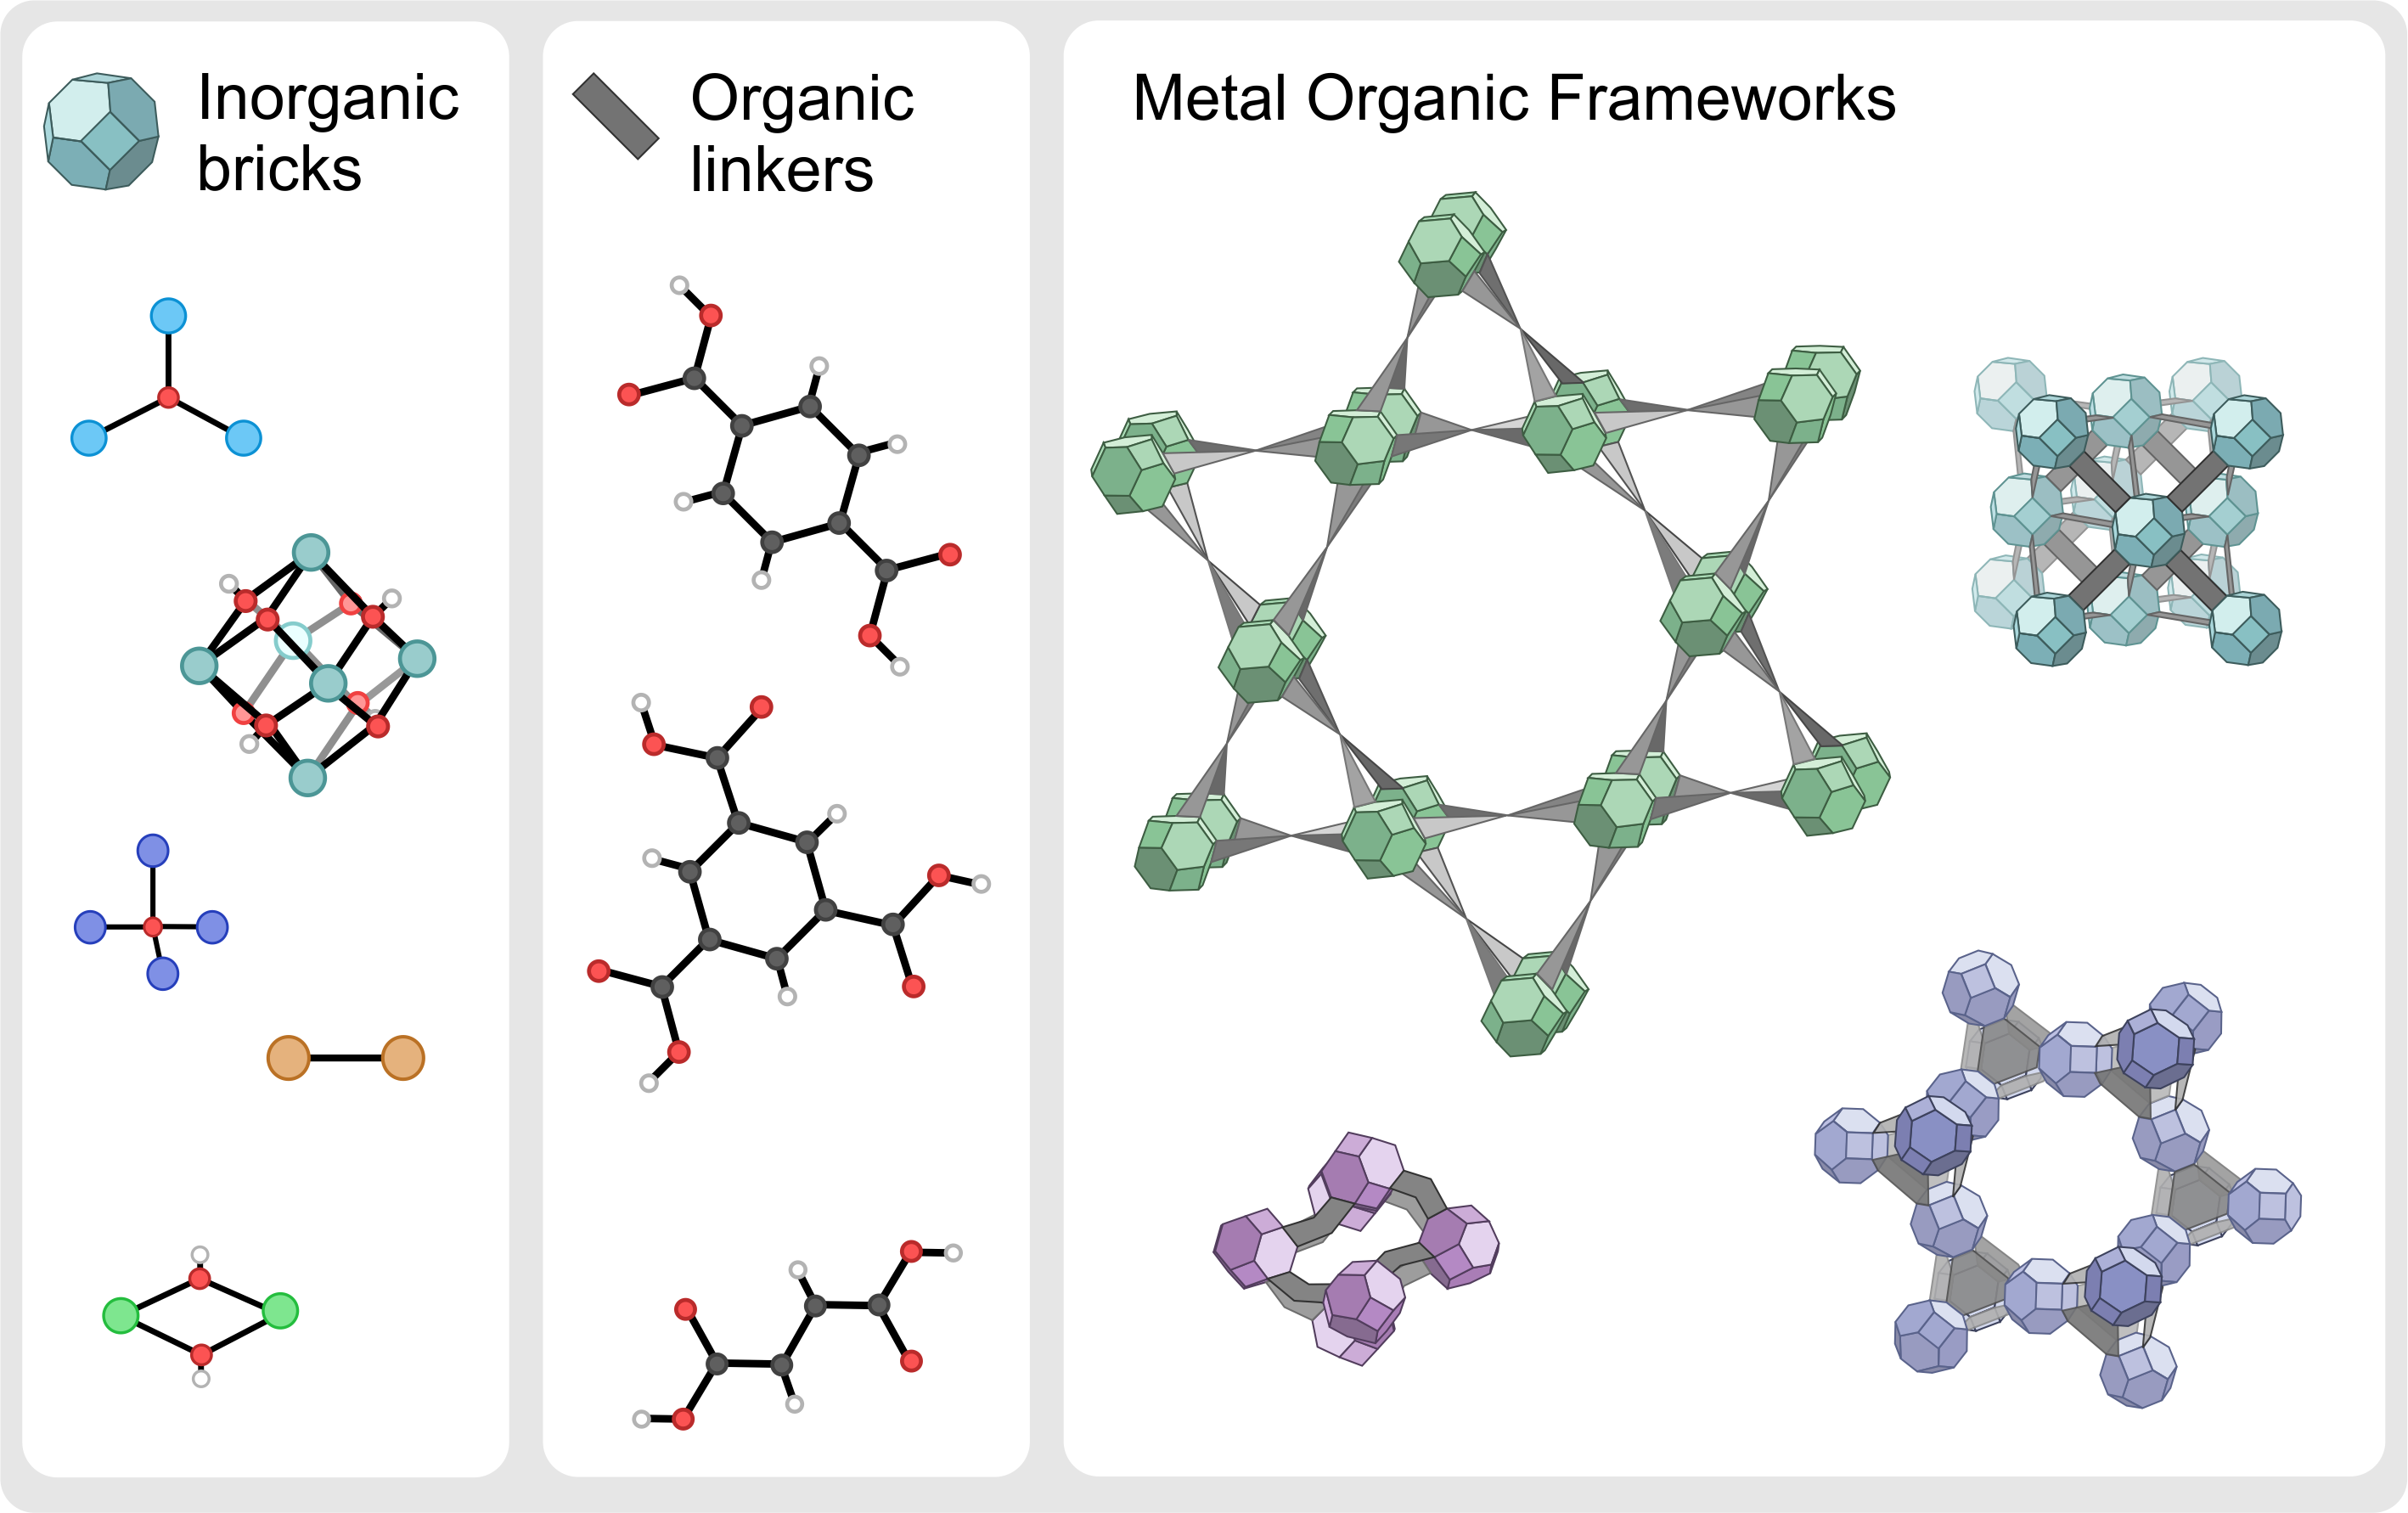
\includegraphics[width=1.0\textwidth]{MOFs}
	\caption{Schematic representation of the building block design in Metal-Organic Frameworks (MOFs). Left panel: some examples of inorganic bricks; middle panel: some examples of organic linkers; right panel: some MOFs with different topologies, pore size and shape}
	\label{fig:MOFs}
\end{figure}

\section{Metal Organic Frameworks}
Metal organic frameworks (MOFs) are one of the most intriguing class of materials of current science. These promising materials, first called 'porous coordination polymers' (PCPs) were discovered in the late 50's, but only at the end of the century with the works of Robson\cite{batten1995two,hoskins1990design}, Kitagawa\cite{kitagawa1991synthesis, kitagawa1993synthesis}, Yaghi\cite{yaghi1995hydrothermal} and Ferey\cite{riou1998hybrid}, the scientific community started to understand their full potential. If at first these materials were seen as a laboratory curiosity, with the focus on the discovery of new structures, in the last few decades, the field has seen an incredible explosion in scientific and industrial interest, with new applications being continuously explored\cite{furukawa2013chemistry}. MOFs are hybrid nanoporous materials that are composed by metal or metal--oxo clusters connected by multitopic organic linkers, to form multidimensional pore structures. Compared to the already established zeolites, MOFs can be constructed without templating agents, with a far greater number of metals and with an exceptional structural diversity. In fact, their particular building block design (Fig. \ref{fig:MOFs}), that makes use of secondary building units (SBUs), allows the creation of an almost infinite number of crystalline structures with different topology and chemical composition. In principle, the nature of the SBUs and their association can be finely tuned\cite{stock2011synthesis}, allowing control on properties such as pore shape and size, functionalization, surface area, or response to chemical and physical stimuli\cite{zhou2014metal,zhou2012introduction}. Moreover, multiple physical or chemical functionalities can be integrated in the crystals at the same time\cite{li2016applications}. 
\npar
Following the nomenclature proposed by Kitagawa, we can differentiate between three generations of porous systems\cite{kitagawa1998functional}. First generation MOFs are defined as having a guest--molecules supported pore system that collapses when these are evacuated, and for this reason found very limited use for practical applications. Those of second generation are more robust and have permanent porosity that is retained even in absence of guest molecules. These materials show high potential for catalysis and other applications and are the main object of this dissertation. Finally, third generation MOFs are characterized by flexible pores that can reversibly change shape with the presence of guest molecules, or upon certain stimuli, such as temperature or pressure. Matsuka et al.\cite{matsuda2004guest} identified five types of response mechanisms in MOFs, denoted as shrinking, expanding, reshaping, swelling and gate opening or closing. A perspective on the types of stimuli that can induce responsive in MOFs has been reported in the work of Coudert \cite{coudert2015responsive}.
%
%
\begin{figure}[htbp]
	\centering
 	\includegraphics[width=1.0\textwidth]{mof-applications}
	\caption{Schematic representation of some of the numerous MOF applications.}
	\label{fig:mof-applications}
\end{figure}
%
%
\npar
The tunability of MOF structures, along with their high cristallinity, metal content and porosity, allows their application in different industrially relevant fields, such as catalysis, gas storage and separation, drug delivery or sensing, as displayed in Fig. \ref{fig:mof-applications}. More specific applications are being further explored, such as warfare agents decomposition, magnetic applications, or membrane separation. 
After the discovery of MOFs, with their tunability and ease in functionalization, the study of their application in catalysis followed naturally, and was one of the earliest documented applications\cite{Fujita1994}. 
Their high porosity, in particular, allows chemical species to diffuse in the pores and access the active sites, and the high metal content offers the possibility to have many guest interactions sites. Exploiting this property, a plethora of MOFs has been synthesized possessing unsaturated metal sites within the pores which offer different Lewis acidity. In this sense, provided the structures are stable at reaction conditions (i.e. no leaking is observed), MOFs can be considered true heterogeneous catalysts, where the active sites are inherent part of the framework. A recent review on the topic can be found in refs.\cite{rogge2017metal, yang2019catalysis}.
%
\begin{figure}[!htbp]
	\centering
 	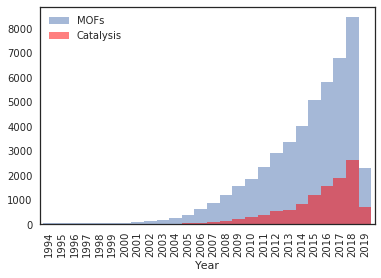
\includegraphics[width=0.8\textwidth]{citation_report}
	\caption{Number of publications on MOFs and catalysis in MOFs by year showing the importance of catalysis in MOFs as indicated by Web of Science)}
	\label{fig:citation_report}
\end{figure}
%
\subsection*{Post--synthetic modification}
One of the most intriguing concepts is the isoreticular synthesis, by which inorganic or organic SBUs can be replaced by topologically identical (or similar) building blocks, giving rise to whole MOF families which derive from a specific precursor and span a range of pore size and functionality. For instance, the pore size can be significantly increased up to the mesoporous range by using longer isoreticular linkers, such as in the IRMOF series\cite{eddaoudi2002systematic}. When it is not possible to introduce functionalities with direct synthesis, post--synthetic modification (PSM) \cite{wang2009postsynthetic}, which makes use of the building block design, has become a well established procedure that allows the preparation of MOF materials with specific chemical composition. 
Via this technique, it is possible to modify the crystal after the synthesis, allowing to finely tune the properties of the material. PSMs include encapsulation of guest molecules or nanoparticles in the pores, modifications of the linkers without breaking the metal--ligand bond, or post synthetic exchange (PSE) of linkers and metals, where building blocks are dynamically exchanged. 
PSE can also involve terminal ligands, or ligands adsorbed on the bricks that do not function as linkers, such as modulators. This way, building blocks can be exchanged, but also eliminated to create vacancies if the stability of the material does not prohibit it. For this reason, PSM has been used as an efficient strategy to introduce defective sites in MOFs. Furthermore, defect--containing MOFs have become an active field in MOF research, as defect sites can play a key role in the performance of the material, as will be shown later. 

\subsection*{Zr--based MOFs}
%%
\begin{figure}[!htbp]
	\centering
 	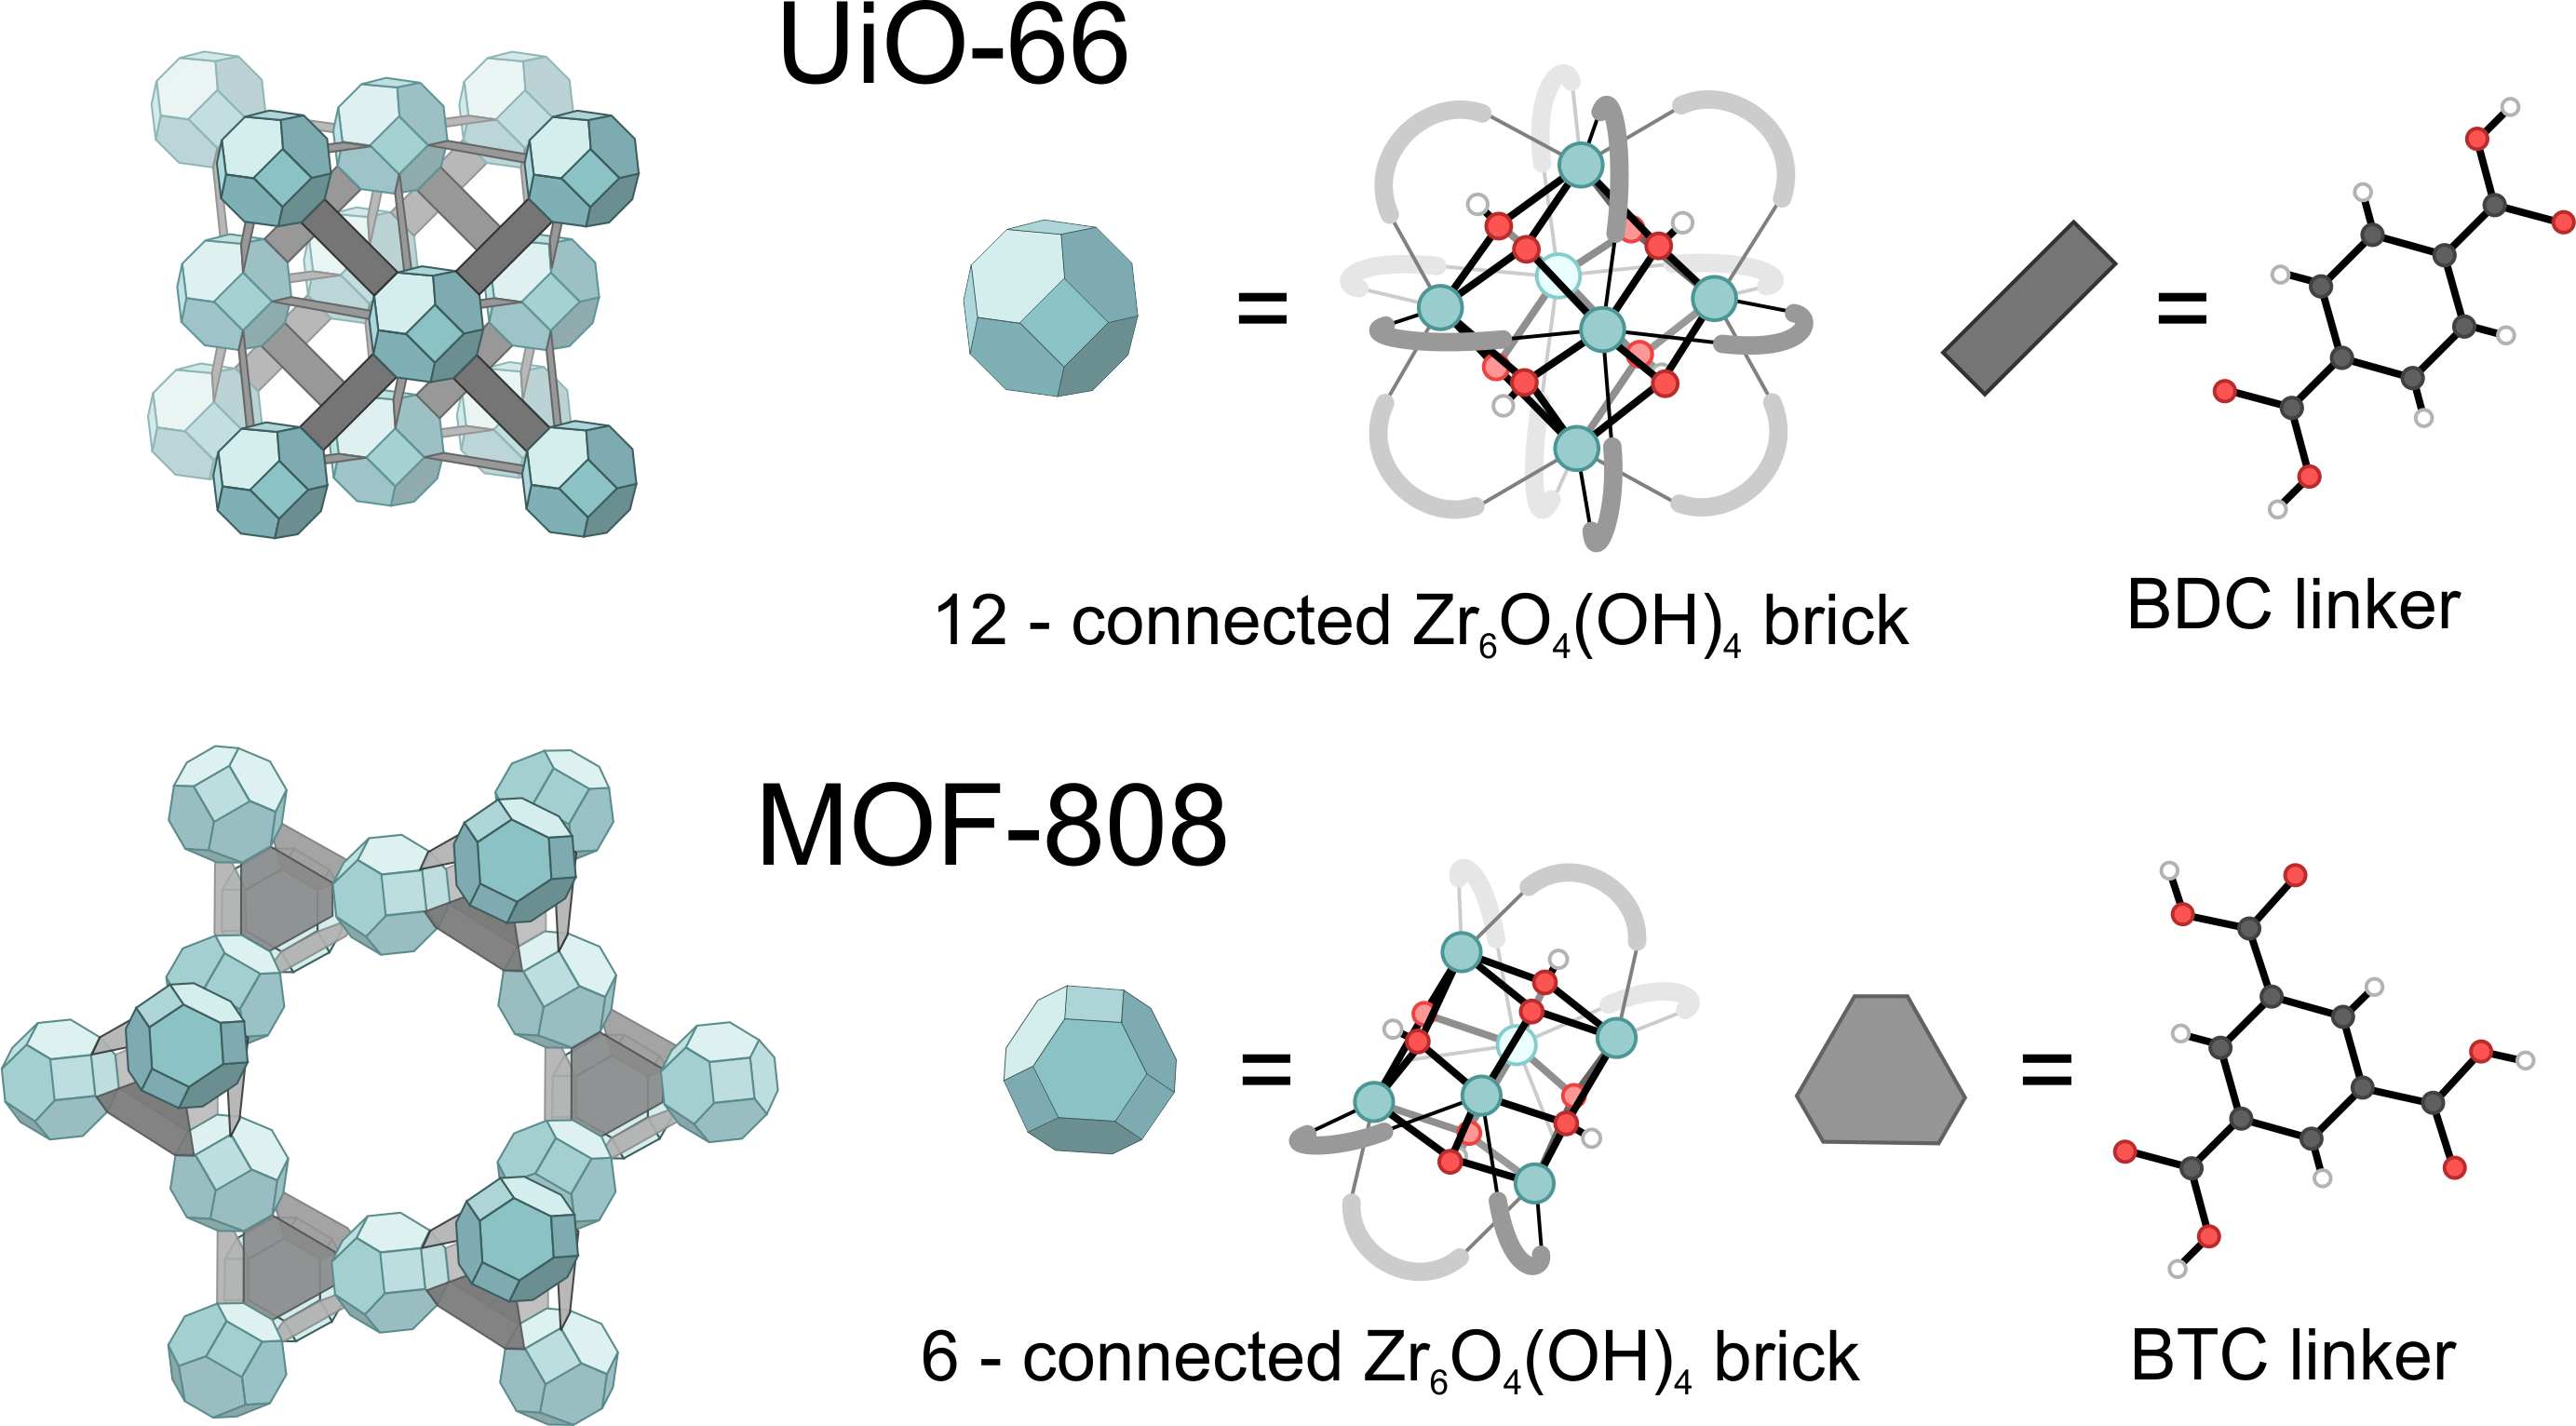
\includegraphics[width=1.0\textwidth]{Zr-MOFs}
	\caption{Structure of UiO--66 (top) and MOF--808 (bottom), the two Zr--MOFs investigated in this work of thesis.}
	\label{fig:Zr-MOFs}
\end{figure}
%%
In general, to function at operating conditions, materials need to retain their thermal, mechanical and chemical stability at those conditions. For instance, mechanical stability is needed when compressing MOF in pellets or other shapes for industrial processes\cite{chapman2009pressure}, while chemical stability is crucial for any application, such as drug delivery, molecular separation, or catalysis\cite{horcajada2010porous}. Catalysis often also requires thermal stability, as the materials must be able to resist harsher conditions for certain processes such as in petrochemistry. 
However, the metal--ligand coordination bond that makes MOFs so tunable is also regarded as one of their main drawbacks\cite{keskin2010can, canivet2014water, kizzie2011effect}, as it is responsible for the lower structural stability when compared to already established nanoporous catalysts such as zeolites. For example, the first synthesized MOFs such as \ce{Cu2+} trimesate HKUST-1, or MOF-5, composed by \ce{Zn2+} clusters and BDC linkers were degraded by water even at mild conditions\cite{greathouse2006interaction, low2009virtual, kaye2007impact, decoste2013effect}. 
\npar
Recently, a class of robust MOFs have been synthesized showing an unprecedented stability\cite{furukawa2014water}. Zr--based MOFs\cite{bai2016zr} which exploit the robustness of the Zr--O bond, show an outstanding stability and are at present time one of the most studied classes of MOFs. Moreover, zirconium is an ubiquitous metal that is present in biological systems and has low toxicity, as well as limited cost. This makes these materials particularly promising for applications in catalysis, gas sorption, and drug delivery. An overview of the plethora of possible structures that can be synthesized with different inorganic SBUs can be found in a recent review by Bai \textit{et al.} \cite{bai2016zr}.
\npar
The vast majority of these materials is characterized by Zr(IV) atoms in a high coordination state (Fig. \ref{fig:Zr-MOFs}), which interact strongly with the oxygens of carboxylate linkers of various topology, and are the focus of this thesis. These MOFs are characterized by a \ce{Zr6O4(OH)4} cluster in which each of the 6 zirconium atoms is connected to 4 oxygen atoms (two $\mu_3$--OH and two $\mu_3$--O), each of which is in turn connected to three zirconium atoms, forming a polyhedron. Each zirconium atom can form 4 other bonds with ligands, accommodating up to 24 metal--ligand bonds per cluster. Every zirconium atom can therefore form a total of 8 coordination bonds oriented in a square--antiprismatic geometry, yielding a rich range of possible structures that can be synthesized with connectivity ranging from 12, as in UiO--66\cite{cavka2008new}, to 6 as in MOF--808\cite{furukawa2014water} (see Fig. \ref{fig:Zr-MOFs}). The dual Lewis acid/base nature of the Zr--carboxylate bonds, along with the high metal oxidation state, gives rise to strong interactions between the SBUs, thus allowing processes such as PSM without compromising the stability of the structures. The stability of Zr--based MOFs depends on the connectivity between the inorganic and organic SBUs, as well as the number of zirconium--ligand bonds that define the structure\cite{bai2016zr}. However, open metal sites in these materials are present only when the connectivity of the linkers is less than 12. Zirconium atoms that remain undercoordinated in these materials are Lewis acid sites where reactants can adsorb and that can function as catalytic centers.

\subsection*{UiO--66}
The precursor of the whole class of Zr--based MOFs is the Zr--therephtalate based UiO--66, which was first synthesized at the Universiteit i Oslo (UiO) by Lillerud and coworkers\cite{cavka2008new}. This material is characterized by an extremely high connectivity that gives rise to an exceptional structural stability, which makes UiO--66 one of the most widely investigated MOFs up to date. In this material, each \ce{Zr6} SBU is connected to 12 therephthalate (or benzenedicarboxylate (BDC)) linkers forming a cubic close packed structure with a space group F\={m}3m, No. 225. In this structure there are two different cavities of octahedral and tetrahedral shape, with window sizes of 10 \AA\ and 25 \AA, respectively. Each octahedral cage shares triangular windows with eight tetrahedral cages. 
This results in an extremely robust material which is stable up to 648 K and in a broad range of protic and aprotic solvents and pH conditions. Moreover, the \ce{Zr6O4(OH)4} bricks be reversibly dehydrated upon thermal treatment at temperatures between 523 and 573 K. Up to two water molecules can be formed this way, yielding a \ce{Zr6O6} brick, where the zirconium atoms have a coordination of 7\cite{valenzano2011disclosing}. 
\npar
A whole family of isoreticular MOFs can be derived from UiO--66 by using linkers of different size, spanning from fumaric acid\cite{wissmann2012modulated} up to terphenyldicarboxylic acid\cite{schaate2011modulated}, allowing to significantly tune pore size and surface area. Interpenetrated MOFs with UiO--66 topology have been also reported if longer linkers are used\cite{schaate2011porous}, with a decrease in surface area. Moreover, different functional groups can be appended to the phenyl rings, such as bromo, amino, nitro, or naphthalene. Garibay and Cohen showed that UiO--66--\ce{NH2} can be further modified to yield new functionalized frameworks \cite{garibay2010isoreticular}. Also the inorganic SBUs can be modified, for instance introducing titanium or hafnium\cite{kim2012postsynthetic}. The exceptional thermal and chemical stability of UiO--66, along with its high connectivity, allows all these modifications of the structure, and for this reason, this material is often considered as a perfect MOF archetype, where new techniques can be tested. 

\begin{figure}[!htbp]
	\centering
 	\includegraphics[width=1.0\textwidth]{defectiveuio}
	\caption{Representation of the UiO--66 material with missing linkers and clusters displayed in red. In this dissertation, we mainly focus on missing linkers.}
	\label{fig:defectiveuio}
\end{figure}

\subsubsection*{Defects}
%chap 11 of book from Garcia
In theory, the perfect crystalline UiO--66 structure, where every zirconium atom is 8--fold coordinated, does not possess undercoodinated Lewis acid sites available for catalysis. However, it became clear that the synthesized UiO--66 showed a behavior that deviated from the theory and pointed towards the presence of defective sites, such as symmetry--forbidden reflections in the PXRD pattern, metal--linker ration obtained by thermogravimetric analysis (TGA), higher than expected surface area, appearance of O--H stretching bands in the FTIR spectrum etc. \cite{shearer2014tuned, valenzano2011disclosing}. It has been generally accepted that the material contains defects in the form of missing linkers or clusters (Fig. \ref{fig:defectiveuio}), and that these are not only naturally occurring during synthesis, but their number can easily be tuned by adapting the synthesis conditions, such as temperature and type of modulator\cite{wu2013unusual, shearer2016defect}.
\npar
Defects can influence the material properties by a large extent. The beneficial role of defects in UiO--66 has been explored in many applications such as gas storage and separation\cite{wu2013unusual, ren2014modulated}, sensing\cite{stassen2016towards}, drug delivery\cite{cunha2013rationale} and catalysis\cite{vermoortele2013synthesis, rogge2017metal}. 
Following the classification proposed by Sholl, these defective sites in MOFs can be either point vacancies (such as missing linkers or clusters) or extended ones such as in the case of a surface \cite{sholl2015defects} or a region in the material. At low defect concentration, a random distribution of isolated point defects can be found, whereas at higher concentrations clustering could occur, if the presence of a vacancy is influenced by other vacancies in proximity. This complexity makes the study of defective sites and disorder a current challenge in MOF research. In particular, the control of their effect on heterogeneous catalysis is heavily limited if their location, type and dispersion are unknown. This randomness can be partially limited by judicious defect engineering during and post--synthesis which is in turn dependent on their understanding at the molecular level. In order to identify and characterize defects in MOFs, it is particularly important to obtain atomic scale resolution on the defect sites and understand how they impact certain properties.
\npar
The physical properties of defective UiO--66 differ according to the number of defects and their location, as has been extensively studied both theoretically and experimentally. A decrease in the connectivity in the structure will naturally lead to a decrease in stability of the material, but the extremely high connectivity of UiO--66 allows the presence of numerous missing linkers or cluster without loss of crystallinity. 
In this context, Rogge et al. report the influence of all possible configurations of one to two linker vacancies on the stability of UiO-66, showing that the equilibrium volume is not affected by such vacancies \cite{rogge2016thermodynamic}. However properties such as bulk modulus and loss--of--crystallinity pressure, which in turn influence the stability, are affected by the relative missing linker configuration. 
De Vos et al.\cite{devos2017missing} reports the electronic properties for all possible configuration of defective UiO--66 with up to three missing linkers, showing that some configurations are energetically more stable than others, and that the number and position of missing linkers affect the band gap of the material. From these studies performed on small unit cells it is already clear that the number of possible defective configurations can be extremely high, and it is still unclear to what extent such point defects are disordered in the material. A regular distribution of point defects that involve missing clusters can lead to different phases in the material, from fcu (non-defective), to bcu (missing linkers with open channels), reo (missing clusters) to scu (missing linkers and missing clusters). Missing clusters could in principle increase the catalytic activity of the material more than missing linkers due to the larger pore size. Recently, Cliffe et al. \cite{cliffe2014correlated} showed in a combined theoretical-experimental work that missing clusters on UiO-66(Hf) were correlated and formed nanodomains in the material, characterized by a reo phase, shedding light into the complexity of modeling disorder in nanoporous material. 

\subsubsection*{Active sites for catalysis on UiO--66}
One of the breakthroughs of MOF research was the discovery that UiO--66 could contain a high number of open metal sites. As reported earlier, active sites for catalysis in UiO--66 and other Zr--MOFs are present when the zirconium connectivity is decreased from its equilibrium value of 8. 
\npar
%active sites by defects
A first way to obtain coordinatively unsaturated zirconium sites is by creation of defects, in the form of missing linkers or clusters. The inherent vacancies in UiO--66 bring unsaturated zirconium Lewis acid sites\cite{wu2013unusual, shearer2014tuned, vermoortele2013synthesis, vandichel2015active, liu2016probing} and at the same time enable the reactants accessibility to the sites, increasing the pore size. The synthesis of defective UiO--66 can be performed via modulators such as formic acid or trifluoroacetic acid (TFA), that are competing with BDC linkers in binding to the inorganic SBU. 
Vermoortele et al. first showed in a dual computational--experimental study that the Lewis catalyzed cyclization of citronellal can only be done on UiO--66 in case of missing linkers\cite{vermoortele2012electronic}. For Meerwein reduction, another Lewis catalyzed reaction, the catalytic activity of UiO--66 could be significantly increased by making use of TFA, that introduced a large number of linker vacancies. Additionally, the non-modulated material that contained only a small number of defects showed nearly no catalytic activity\cite{vermoortele2013synthesis}. Such relationship between catalytic activity and amount of defects has been reported for different Lewis catalyzed reactions giving evidence that the catalytic centers are located on the defective sites. 
\npar
The molecular characterization of the defective sites on UiO--66 has been an ongoing research interest in MOF literature. Lillerud and coworkers \cite{oien2014detailed} reported that when linker vacancies were present, XRD characterization of the material showed two type of Zr--bonded oxygen atoms. The first type was BDC oxygen, and the other was associated to water species coordinated to the zirconium on the defect site. Still from XRD measurements, the group of Yaghi \cite{trickett2015definitive} proposed that the two Zr--bonded oxygens belonged to physisorbed water molecules and that the charge compensating species was a hydroxyl group. Insight from molecular simulations helped to shed light into the characterization of the active sites at the molecular level. Ling and Slater \cite{ling2016dynamic} performed MD simulations starting from such structure and showed a progressive stabilization towards a structure where the two adjacent zirconium atoms were coordinated to a physisorbed water molecule and a hydroxyl group, as shown in Fig. \ref{fig:bronsted-lewis-uio}. These sites has been also confirmed by a comprehensive computational study of different adsorption possibilities of up to three water molecules on defective UiO--66 performed by Vandichel et al. \cite{vandichel2016water} and by simulations performed in this work of thesis. 
Such species are strongly interacting with the zirconium atoms and are sources of Br\o{}nsted sites that can play an active role in catalytic processes involving proton transfers, as will be shown in \textbf{PAPER I} and can in principle be considered as part of the catalyst. Serre and coworkers report that a hydrogen bonded network that spans the octahedral and tetrahedral cages is responsible for the high proton conductivity showed by UiO-66 at high temperatures \cite{borges2016proton}. Kitagawa et al. showed the positive role of defects in proton conductivity in the UiO-66 material, as defective sites provide both larger pores and zirconium-bonded water species that are proton donors \cite{taylor2015defect}. Farha and coworkers make use of the acidic protons belonging to physisorbed water molecule on the defective site for the quantification of defects, by means of potentiometric titration \cite{klet2016evaluation}. The chemistry associated with the hydroxyl group face topology changes on the inorganic SBU has been investigated by Yang et al.\cite{yang2016tuning}. The interaction between defect--coordinating water molecules and zirconium atoms is strong, and UiO--66 can be partially hydrolized\cite{decoste2013stability} while retaining its stability, as will be further discussed in this dissertation.
\npar
The defect--coordinating species can be removed by thermal activation at T $>$ 423 K (\textbf{PAPER I}). The more loosely bonded physisorbed water is the first to leave the defective site, followed by the chemisorbed water. The dehydrated active site obtained this way is missing a $\mu_{3}$--OH proton and has two 7--fold coordinated zirconium open metal sites as shown in Fig. \ref{fig:bronsted-lewis-uio}. 
\npar
%active sites by dehydration
The second activation process by which open metal sites can be created on UiO--66 is the reversible dehydration of the \ce{Zr6O4(OH)4} cornestone to obtain \ce{Zr6O6} by removal of up to two water molecules performed at a temperature range between 523 and 573 K \cite{valenzano2011disclosing}. The 7--fold coordinated zirconium atoms are Lewis acid sites, but the large pores created by linker vacancies are missing, and the active sites are less accessible than in the defective material. 
%The presence of these species give a dual Bronsted--Lewis catalytic nature to UiO--66.
%The electroneutrality of the structure makes it so that at least one negatively charged species has to be coordinated to the inorganic SBU. 
\begin{figure}[!htbp]
	\centering
 	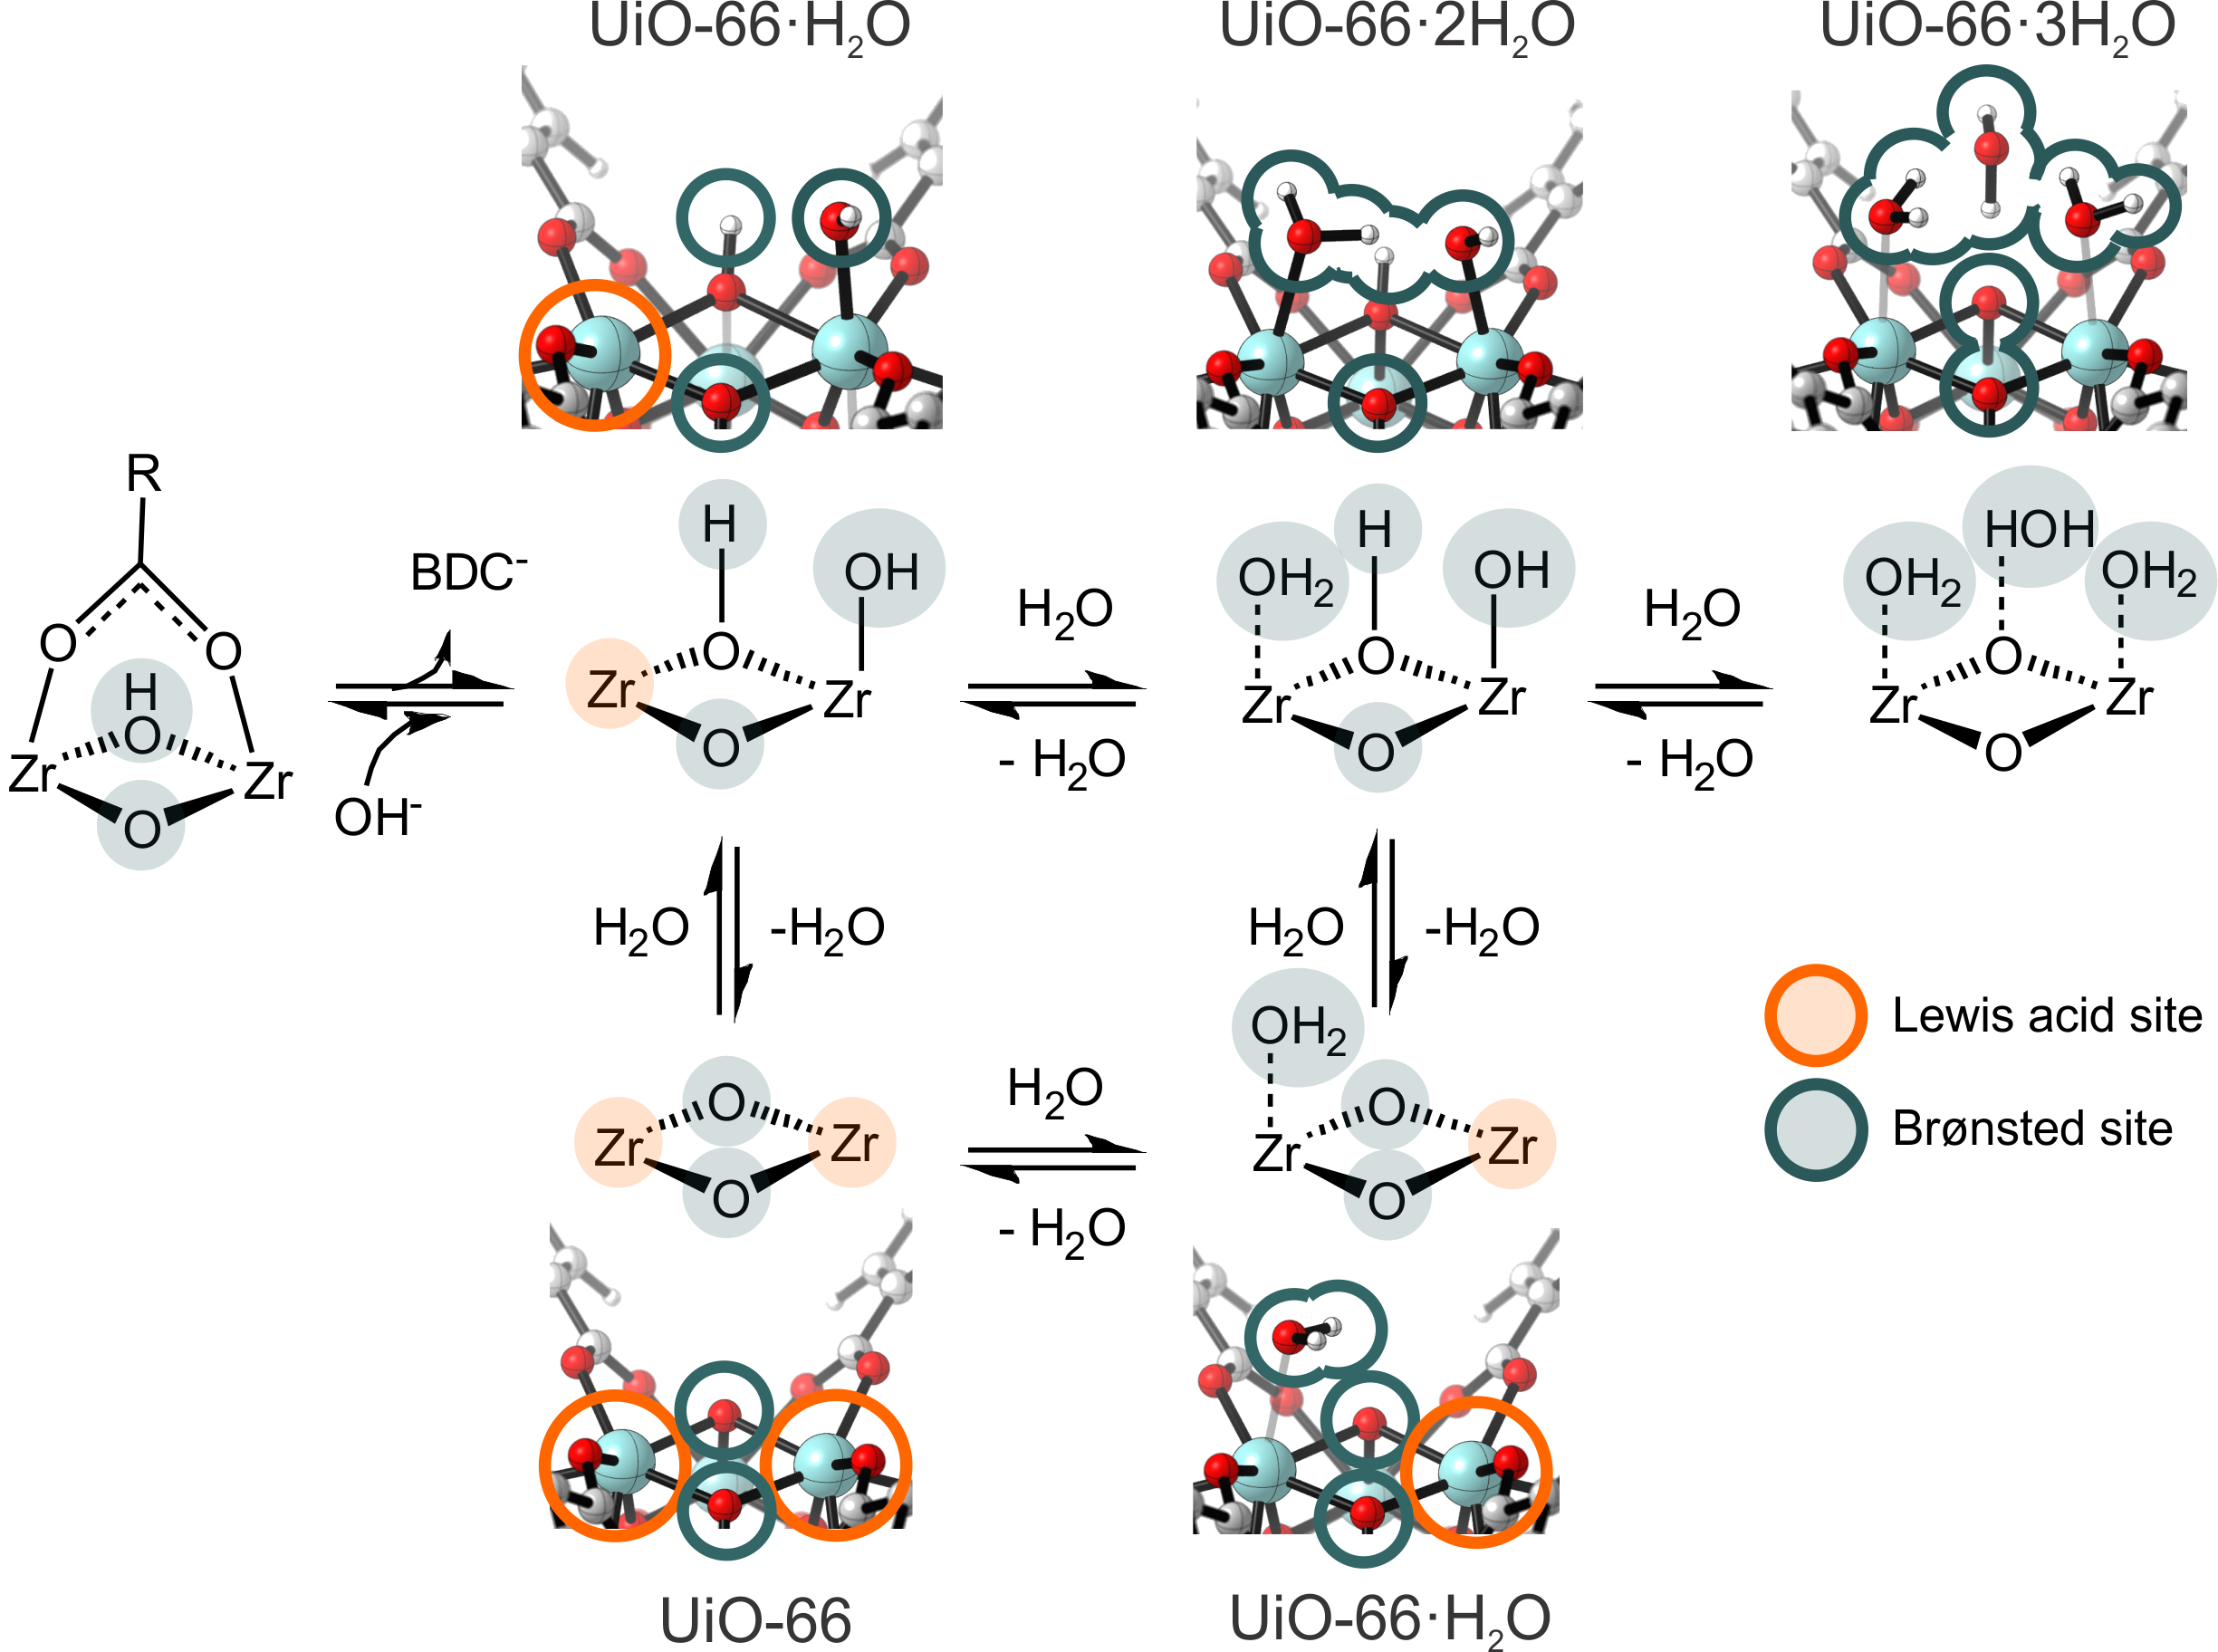
\includegraphics[width=1.0\textwidth]{bronsted-lewis-uio}
	\caption{Lewis and Br\o{}nsted sites that are created when a linker is removed from the UiO--66 zirconium brick, with different number of coordinated water molecules.}
	\label{fig:bronsted-lewis-uio}
\end{figure}
\subsubsection*{Functionalization}
As anticipated earlier, the nature of the active sites can also be influenced by linker functionalization \cite{kandiah2010synthesis, kandiah2010post, kim2012discovery}. 
The presence of electron--donating substituents showed an increase in catalytic activity for jasminaldehyde condensation \cite{vermoortele2011amino}. The effect of other functional groups was subsequently studied by the same authors for Lewis catalyzed citronellal cyclization \cite{vermoortele2012electronic}, who report a positive effect of electron--withdrawing groups. The beneficial role of amino groups was reported as well by Timofeeva et al. \cite{timofeeva2014effects} for acetylisation of benzaldehyde, as well as by Cirujano et al \cite{cirujano2015zirconium, cirujano2015conversion} for esterification. The electron donating effect of amino groups would in principle lead to a decrease in the Lewis acidity of the defective zirconium atoms, lowering the reaction rate. Therefore, a change in mechanism in the presence of BDC--\ce{NH2} was hypothized. However, Hajek et al. further studied aldol condensation in a computational work\cite{hajek2015mechanistic}, and reported a beneficial, but passive role of amino groups, which is further confirmed in \textbf{PAPER I} for Fischer esterification. 

\subsection*{Active sites on MOF--808}
MOF--808, formed by the inorganic \ce{Zr6O4(OH)4} cornestone and trimesate (BTC) linkers, represent the least connected MOF in the Zr--MOF family \cite{furukawa2014water}, and its brick can be regarded as an extreme case of defective UiO--66. The rigid BTC tritopic linkers stabilize the structure and yield exceptionally wide channels which are required for the diffusion of substrates. The octahedral crystals contain 6 BTC linkers per inorganic node and are characterized by a \textit{spn} topology. 
In the material, each zirconium atom is bonded to four oxygens from the inorganic brick and two oxygens from the BTC linkers. The other two bonds that are needed to reach the total coordination of 8 are provided by species present in solution that do not contribute to the framework connectivity. 
\npar
In the as--synthesized material, the zirconium atoms are capped with the relative mobile formate modulator. The material at this stage does not contain catalytically active sites and must be activated by post--synthetic treatment. By hot filtration, the formate groups can be eliminated and replaced by water and hydroxyl groups. In the catalytically active material, each brick is connected to six BTC linkers, six water molecules and six hydroxyl groups, and possesses a high number of potential Br\o{}nsted sites. Klet et al. report the presence of four different types of protons in the material \cite{klet2016evaluation}. Lewis acid sites can be created by thermal activation, similarly as in UiO--66. In this case, hydroxyl groups remain connected to the zirconium atoms and the material possesses both Lewis and Br\o{}nsted sites. The hydroxyl groups could also be used as anchors to incorporate new features, for instance by molecular docking of a single-site catalyst to immobilize it on a MOF-scaffold. MOF--808 is a promising catalyst that is still less studied than UiO--66, but has a lot of potential for possible applications. For instance, it shows a higher catalytic activity for certain Lewis catalyzed reactions, such as Meerwein-Ponndorf-Verley (MPV) reduction \cite{plessers2016zr, mautschke2018catalytic}. 
Moreover, MOF--808 represents the first evidence of a superacid in MOFs, showing superacidity after post--synthetic treatment with sulfuric acid \cite{jiang2014superacidity}.

\section{Outline and goal of the thesis}
In this chapter, the characteristics of MOFs that make them appealing as catalysts have been shown, as well as the current challenges that MOF research is facing. The properties of catalytically active sites on defective UiO--66 and MOF--808 were studied by means of molecular modeling techniques. Molecular modeling can give fundamental insight into the properties of MOFs, and at present time a plethora of different techniques are available for this purpose. To model processes in MOFs, knowledge of both power and limitations of these methods and experimental insight into the scientific question are required to find the appropriate combination of techniques.\\
This PhD thesis is organized as follows:
\begin{itemize}
\item In Chapter 2, a theoretical overview of the state of the art modeling techniques is given. Particular attention is drawn on how these techniques can be applied in the case of MOF materials to obtain insight into structural and catalytic properties at operating conditions.
\item In Chapter 3, the main results of this PhD thesis are summarized. The links between theory and experiment are highlighted throughout the chapter. All results are the result of fruitful collaborations and have been published in international peer--reviewed journals. 
\item In Chapter 4, the main conclusions of this thesis work, as well as perspectives on future research are given.
\end{itemize}

\clearpage{\pagestyle{empty}\cleardoublepage}
